\chapter{Open Quantum Systems}



%
In general it is impossible to prevent any quantum system, such as an atom/molecule or superconducting qubit, from coupling to its surroundings or the environment \cite{QuNoise}. This leads to phenomenon of decoherence which represents loss of information from a system to its environment. Since the environment typically consists of a several degrees of freedom that we are unable to track or control, either experimentally or theoretically, the coherence is usually irretrievably lost. Due to decoherence the usual steady state of the system is a statistical mixture. Such a mixture necessitates the description of the system via a density matrix instead of the usual state vector describing a wavefunction. The formalism of open quantum systems (OQS) is employed to study the behavior of such systems of interest interacting with extraneous degrees of freedom. The typical OQS methods partition the full Hilbert space into a system space $S$ (atom/qubit), and a reservoir space $R$ (representing the environment). Since we are only interested in the dynamical behavior of degrees of freedom that belong to the system $S$, the reservoir degrees of freedom, $R$, are ultimately traced over; a procedure called partial trace. Figure \ref{Fig:CPTP} gives a schematic description of this procedure, where the ultimate goal is to get a dynamical map $V(t)$ describing the evolution of the reduced system.
%
\par
%
In the following sections, we present a detailed derivation of a widely used form of this dynamical map relevant for `weak' system-reservoir coupling (perturbative regime), that leads to an equation of motion for the reduced system called Gorini– Kossakowski– Sudarshan– Lindblad (GKSL) equation. As a means of demonstration, we use this to describe a single qubit weakly coupled to an environment, consisting of a collection of independent oscillators, and derive optical Bloch equations describing the dynamics of a driven-dissipative qubit.

%derive the quantum master equation for the atom in the regime of weak atom-environment coupling. We next make a two-level approximation for the atom (now a `qubit'/qubit) and obtain optical Bloch equations describing the evolution of a driven-dissipative qubit.
%
%Because of the weak-coupling assumption, it is assumed that state of the reservoir, $R$, is time independent. That is  $\langle \dot{b} \rangle \approx 0$ which is sometimes called the quasi-static bath condition. What this measn is the timescale of the changed caused by the "weak" interaction is so slow, compaired to internal dynamics of the reservoir, thus it remains in its equilibrium stationary state. When the reservoir is quasi-static it can be adiabatically eliminated to get an engineered dissipation rate.
%
\begin{figure}
\begin{tikzcd}[column sep=4cm]
\chi (0)= \rho_{\mathcal{S}}(0) \otimes \rho_{\mathcal{R}}(0) \arrow{r}{\text{Unitary Evolution}} \arrow{d}{tr_{\mathcal{R}}}  & \chi(t) =  \hat{U}(t) \left( \rho_{\mathcal{S}}(0) \otimes \rho_{\mathcal{R}}(0) \right) \hat{U}(t) \arrow{d}{tr_{\mathcal{R}}}\\
\rho_{\mathcal{S}}(0) \arrow{r}{\text{Dynamical Map}} & \rho_{\mathcal{S}}(t)=V(t)\rho_{\mathcal{S}}(0)
\end{tikzcd}
\caption{Two potential ways of partial trace over the environment. Here $\chi(0)$ represents the full density operator of system and reservoir, while $\rho_{S}$ describes the density operator of the reduced system.}
\label{Fig:CPTP}
\end{figure}
%
%%%%%%%%%%%%%%%%%%%%%%%%%%%%%%%%%%%%%%%%%%%%%%%%%%
\section{Quantum Master (GKSL) Equation}
%%%%%%%%%%%%%%%%%%%%%%%%%%%%%%%%%%%%%%%%%%%%%%%%%%
%
%When the interaction between the system and reservoir is weak, such that the timescale of evolution caused by the interaction is much slower, the reservoir is called Markovian. Essentially, the reservoir correlation function decay rapidly, will result in the makovian master equation in Lindblad form.
%
Let us consider the Liouville-von Neumann equation in the Schr\"{o}dinger picture
\begin{equation}\label{Liouville-von Neumann}
\dot{\chi} = - \frac{i}{\hbar} [H , \chi],
\end{equation}
which captures the time dynamics of the density operator
\begin{equation}
\chi = \sum_n p_n \left|\Psi_n \>\< \Psi_n \right|
\end{equation}
for both the system and the reservoir, $S+R$. Partitioning the Hilbert space into system and reservoir subspace, the Hamiltonian can be written as 
%
\begin{equation}
H = H_{\mathcal{S}}\otimes I_{\mathcal{R}} + I_{\mathcal{S}} \otimes H_{\mathcal{R}}+ H_{\mathcal{SR}}
\end{equation}
%
where $H_{\mathcal{S}} \in \mathcal{H}_{\mathcal{S}}$, $H_{\mathcal{R}} \in \mathcal{H}_{\mathcal{R}}$, and $H_{\mathcal{SR}}\in \mathcal{H}$ mediates the interaction between the the two subspaces (Fig. \ref{Hilbert_Space}). Typically, the tensor products with the complement space are assumed, and will be henceforth suppressed for brevity of notation.
%
\begin{figure}
\centering
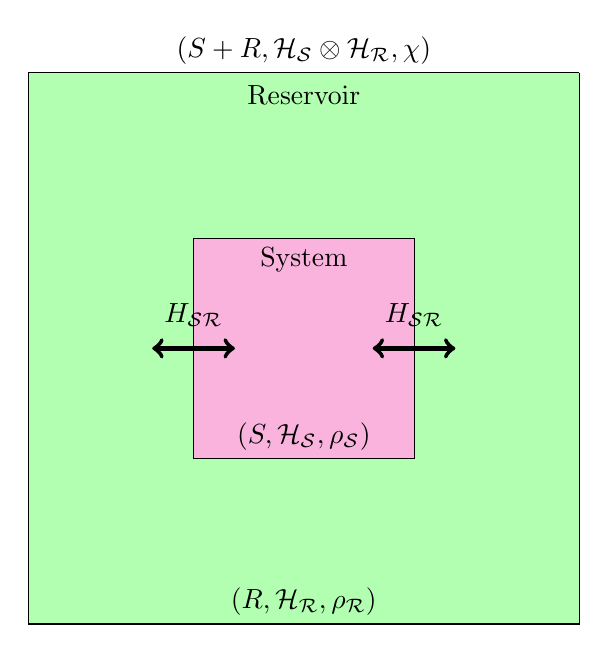
\begin{tikzpicture}[scale=.7]
\draw [fill=green!30] (10,10) -- (0,10) -- (0,0) -- (10,0)--(10,10);
\node at (5,10.4) {\scalebox{1.0}{$\left(S+R, \mathcal{H}_{\mathcal{S}} \otimes \mathcal{H}_{\mathcal{R}}, \chi \right)$}} ;
\draw [fill=magenta!30] (7,7) rectangle (3,3 );
\node at (5,.4) { \scalebox{1.0}{\textcolor{black}{$\left(R, \mathcal{H}_{\mathcal{R}}, \rho_{\mathcal{R}} \right)$}} };
\node at (5,3.4) {\scalebox{1.0}{$\left(S, \mathcal{H}_{\mathcal{S}}, \rho_{\mathcal{S}} \right)$}};
\draw[ultra thick, <->] (2.25,5) -- (3.75,5);
\draw[ultra thick, <->] (6.25,5) -- (7.75,5);
\node at (3,5.6) {\scalebox{1.0}{$H_{\mathcal{SR}}$}};
\node at (7,5.6) {\scalebox{1.0}{$H_{\mathcal{SR}}$}};
\node at (5,6.6) {\scalebox{1.0}{System}};
\node at (5,9.6) {\scalebox{1.0}{Reservoir}};
\end{tikzpicture}
\caption{Partitioning of the full Hilbert space into system and reservoir subspaces.}
\label{Hilbert_Space}
\end{figure}
%
To zoom in on the slow dynamics caused by the interaction $H_{\mathcal{SR}}$, we move into the interaction picture. Defining 
\begin{equation}\label{full_dentity_matrix_interaction_picture}
\tilde{\chi}(t) = e^{i (H_{\mathcal{S}} + H_{\mathcal{R}})t/\hbar} \chi e^{- i (H_{\mathcal{S}} + H_{\mathcal{R}})t/\hbar}
\end{equation}
and taking the time derivative of Eq. (\ref{full_dentity_matrix_interaction_picture}), we obtain
\begin{eqnarray}\label{density_matrix_dynamics_interaction_picture}
\dot{\tilde{\chi} } & = & \frac{i}{\hbar} (H_{\mathcal{R}} + H_{\mathcal{S}} )\tilde{\chi} - \frac{i}{\hbar}\tilde{\chi} (H_{\mathcal{R}} + H_{\mathcal{S}} )+ e^{i (H_{\mathcal{S}} + H_{\mathcal{R}})t/\hbar} \dot{\chi} e^{- i (H_{\mathcal{S}} + H_{\mathcal{R}})t/\hbar} \nonumber \\
& =&  - \frac{i}{\hbar} [\tilde{H}_{\mathcal{SR}}(t) , \tilde{\chi}(t)],
\end{eqnarray}
where
\begin{equation}
\tilde{H}_{\mathcal{SR}}(t) = e^{i (H_{\mathcal{S}}+H_{\mathcal{R}})t/\hbar} H_{\mathcal{SR}} e^{-i (H_{\mathcal{S}}+H_{\mathcal{R}})t/\hbar}.
\end{equation}
The formal solution to this equation is
\begin{equation}\label{Formal_Soltuion_Density_Matrix_Interaction_Picture}
\tilde{\chi}(t) = \chi(0) - \frac{i}{\hbar} \int_0^t ds \, [\tilde{H}_{\mathcal{SR}}(s) , \tilde{\chi}(s)].
\end{equation}
Note that $\tilde{\chi}(0) = \chi(0)$. Substituting the formal solution, Eq. (\ref{Formal_Soltuion_Density_Matrix_Interaction_Picture}), in Eq. (\ref{density_matrix_dynamics_interaction_picture}), we obtain the equation for the full density operator in the interaction picture
\begin{equation}
\dot{\tilde{\chi}}  =  -\frac{i}{\hbar} [ \tilde{H}_{\mathcal{SR}}(t), \chi(0) ] - \frac{1}{\hbar^2} \int_0^t ds \, [\tilde{H}_{\mathcal{SR}}(t), [\tilde{H}_{\mathcal{SR}}(s), \tilde{\chi}(s)]].
\end{equation}
In order to obtain an equation describing dynamics of the reduced system, $S$, we partial trace over the reservoir degrees of freedom
\begin{equation}\label{Exact_density_matrix_dynamics}
\dot{\tilde{\rho}} =  - \frac{1}{\hbar^2} \int_0^t ds \,  tr_{\mathcal{R}} \left\lbrace [\tilde{H}_{\mathcal{SR}}(t), [\tilde{H}_{\mathcal{SR}}(s), \tilde{\chi}(s)]] \right\rbrace.
\end{equation}
Here, $\tilde{\rho}_{\mathcal{S}}(t) = tr_{\mathcal{R}}\left\lbrace \tilde{\chi} (t)\right\rbrace$ and we assumed that
\begin{equation}\label{Traceless_assumption}
tr_{\mathcal{R}}  \left\lbrace [ \tilde{H}_{\mathcal{SR}} (t), \chi(0) ] \right\rbrace = 0.
\end{equation} 
The assumption is true when the reservoir is in the vacuum state; for any general state of the reservoir this can be ensured by adding the term $tr_{\mathcal{R}} \left\lbrace H_{\mathcal{SR}} \rho_{\mathcal{R}} \right\rbrace$ to the system Hamiltonian \cite{StatMethQOI}. At this stage Eq. (\ref{Exact_density_matrix_dynamics}) is exact since no approximations have been made so far.
%However, the dynamics of the density matrix have been cast into a form where reasonable approximations can be made.
%
%ccccccccccccccccccccccccccccccccccccccccc
\subsection{Born-Markov Approximation}
%cccccccccccccccccccccccccccccccccccccccc
%
The first assumption that is made is the system and reservoir begin uncorrelated and remain uncorrelated because $H_{\mathcal{SR}}$ is weak. Furthermore, it is assumed that density operator of the environment is time-independent. This implies,
%
\begin{equation}
\tilde{\chi}(t) = \tilde{\rho}_{\mathcal{S}}(t) \otimes \rho_{\mathcal{R}}. 
\end{equation}
so
\begin{equation}\label{non_markovian_master_equation}
\dot{\tilde{\rho}}_{\mathcal{S}} =  - \frac{1}{\hbar^2} \int_0^t ds \,  tr_{\mathcal{R}} \left\lbrace [\tilde{H}_I(t), [\tilde{H}_I(s), \tilde{\rho}_{\mathcal{S}}(s) \otimes \rho_{\mathcal{R}}]] \right\rbrace.
\end{equation}
Typically correlations (entanglement) between the subsystems build up because of the interaction. Thus we are assuming the reservoir is so large, compared to the system, that it is virtually unaffected by the coupling to the system. This equation is sometimes called the Redfield equation which was developed in the context of nuclear magnetic resonance \cite{IBM}. %For concerns we will considered exclusively reservoir in the thermal state


%At this point   Eq. ()Next $\tilde{\rho}_S(s) \rightarrow \tilde{\rho}_S(t)$ which says that th. This equation is called the Redfield equation, which isn't yet Markovian because it doesn't have so we make a substation, $s=t-\tau$ and extend the limits of integration to infinity.
%\begin{equation}
%\dot{\tilde{\rho}} = - \frac{1}{\hbar^2} \int_0^\infty d\tau \, \,  tr_R \left\lbrace [\tilde{H}_I(t), [\tilde{H}_I(t - \tau), \rho_S(t) \otimes \rho_R.]] \right\rbrace
%\end{equation}

To proceed any further, we have to be more specific about the form of the interaction. Since the interaction acts on both subspaces, without loss of generality, we can decompose the interaction as 
%
\begin{equation}\label{Tensor_Product_Interaction}
H_{\mathcal{SR}} = \hbar  \sum_\alpha A_\alpha \otimes b_\alpha^\dagger + h.c. 
\end{equation}
%
where $b_\alpha^\dagger$ denotes the creation operator for a given oscillator comprising the reservoir. Then moving into the interaction picture, this gives
\begin{equation}
\tilde{H}_{\mathcal{SR}}(t)  =  \hbar  \sum_\alpha A_\alpha(t) \otimes b_\alpha^\dagger(t) + h.c.
\end{equation}
where $A_\alpha(t)= e^{i H_{\mathcal{S}} t / \hbar } A_\alpha e^{- i H_{\mathcal{S}} t /\hbar }$ and $b_\alpha(t) = e^{i H_{\mathcal{R}} t/ \hbar } b_\alpha e^{-i H_{\mathcal{R}} t /\hbar }$. For a reservoir in a thermal state at temperature $T$, the density operator can be written as,
%
\begin{equation}
\rho_{\mathcal{R}} = \frac{1}{tr_{\mathcal{R}} \lbrace e^{-H_{\mathcal{R}} / k T} \rbrace} e^{-H_{\mathcal{R}} / k T}.
\end{equation}
%
where $H_{\mathcal{R}} = \hbar \sum_\alpha \omega_\alpha b_\alpha^\dagger b_\alpha$. We are now able to trace over the reservoir degrees of freedom
%
\begin{align}
\dot{\tilde{\rho}}_{\mathcal{S}} & =  \sum_{\alpha \beta } \int_{0}^{t} d\tau \;  \biggl\lbrace \left[   A_\beta (t-\tau) \tilde{\rho}_{\mathcal{S}} , A_\alpha(t) \right] \left\langle b_\alpha(t) b_\beta(t-\tau) \right\rangle \nonumber \\
& \quad + \left[   A_\beta^\dagger (t-\tau) \tilde{\rho}_{\mathcal{S}} , A_\alpha^\dagger(t) \right] \left\langle b_\alpha^\dagger(t) b_\beta^\dagger (t-\tau) \right\rangle  \nonumber \\
& \quad + \left[  A_{\beta}^\dagger(t-\tau) \tilde{\rho}_{\mathcal{S}} , A_\alpha(t)   \right] \left\langle b_\alpha(t) b_\beta^\dagger(t-\tau)  \right\rangle \nonumber \\
& \quad + \left[  A_{\beta}(t-\tau) \tilde{\rho}_{\mathcal{S}} , A_\alpha^\dagger(t)   \right] \left\langle b_\alpha^\dagger(t) b_\beta(t-\tau)  \right\rangle + h.c. \biggr\rbrace 
\label{Eq:rho1}
\end{align} 
%
To proceed any further we need to evaluate the correlation functions of the reservoir. For a Markovian reservoir, these correlation functions decay more rapidly than any timescale associated with the system. Ideally, they would decay instantaneously i.e. \cite{StatMethQOI}
%
\begin{equation}
\left\langle b_\alpha^{\dagger}(t) b_\beta(s) \right\rangle \sim \delta(t-s).
\end{equation}
%
Calculating the correlation functions explicitly, we find
\begin{eqnarray}
\left\langle b_\alpha(t) b_\beta(t-\tau) \right\rangle & = & \left\langle b_\alpha^\dagger(t) b_\beta^\dagger(t-\tau) \right\rangle = 0 \\
\left\langle b_\alpha^\dagger(t) b_\beta(t-\tau) \right\rangle & = & \gamma_\alpha N( \omega_\alpha ) \delta_{\alpha \beta} \delta(\tau) \\
\left\langle b_\alpha(t) b_\beta^\dagger(t-\tau) \right\rangle & = & \gamma_\alpha (1+N( \omega_\alpha )) \delta_{\alpha \beta} \delta(\tau) 
\end{eqnarray}
where 
\begin{equation}
N_\omega_{\alpha} = \frac{1}{e^{\hbar\omega_{\alpha}/k_B T} - 1}
\end{equation}
is the Bose-Einstein occupation number. Substituting the correlation functions in Eq. (\ref{Eq:rho1}), we obtain
\begin{align}
\dot{\tilde{\rho}}_{\mathcal{S}} & =  \sum_{\alpha } \gamma_\alpha \left\lbrace \left[  A_{\alpha}^\dagger(t) \tilde{\rho}_{\mathcal{S}} , A_\alpha(t)   \right] \left( 1 + N(\omega_\alpha) \right) + \left[  A_{\alpha}(t) \tilde{\rho}_{\mathcal{S}} , A_\alpha^\dagger(t)   \right] N( \omega_\alpha ) + h.c. \right\rbrace \nonumber
\end{align} 
Moving back into the Schrodinger picture using
\begin{equation}
 \dot{\rho}_{\mathcal{S}} = -\frac{i}{\hbar} [H_{\mathcal{S}}, \rho_{\mathcal{S}} ] + e^{-i H_{\mathcal{S}} t} \left( \frac{d}{d t } \dot{\tilde{\rho}}_{\mathcal{S}} \right) e^{ i H_{\mathcal{S}} t }
\end{equation}
we find
\begin{align}
\dot{\rho}_{\mathcal{S}} & = -\frac{i}{\hbar}[H_{\mathcal{S}}, \rho_{\mathcal{S}}] + \sum_{\alpha} \gamma_\alpha \left\lbrace \left[  A_{\alpha}^\dagger \rho_{\mathcal{S}} , A_\alpha   \right] \left( 1 + N(\omega_\alpha) \right) + \left[  A_{\alpha} \rho_{\mathcal{S}} , A_\alpha^\dagger   \right] N( \omega_\alpha ) + h.c. \right\rbrace . \nonumber
\end{align} 
Expanding out the commutators we can write 
\begin{align}\label{Effective_dynamics}
\dot{\rho}_{\mathcal{S}} & = - \frac{i}{\hbar} [H_{\mathcal{S}}, \rho_{\mathcal{S}} ] \\
& \quad +  \sum_{\alpha } \frac{\gamma_\alpha}{2} \biggl[ (1 + N_{\omega_\alpha} ) \left( A_\alpha \rho_{\mathcal{S}} A_\alpha^\dagger + \frac{1}{2} \left\lbrace A_\alpha^\dagger A_\alpha , \rho_{\mathcal{S}} \right\rbrace \right) \nonumber\\
& \quad +  N_{\omega_\alpha}  \left( A_\alpha^\dagger \rho_{\mathcal{S}} A_\alpha +\frac{1}{2} \left\lbrace A_\alpha A_\alpha^\dagger , \rho_{\mathcal{S}} \right\rbrace \right)\biggr]. \nonumber
\end{align} 
We now have have an equation that captures the effective dynamics of the open system $\mathcal{S}$. Typically, $A_\alpha$ is proportional to a lowering operator. This makes the second term describe decay of the system into the reservoir, with a rate proportional $\gamma_\alpha(1+N_{\omega_k})$.  And the third term proportional to absorption of the system from the reservoir.
%
%cccccccccccccccccccccccccccccccccccccccccccccccccc
\section{Optical Bloch Equations}
%cccccccccccccccccccccccccccccccccccccccccccccccccccc
%
We now present a simple example of a driven-dissipative two-level system (a.k.a. qubit), coupled to a reservoir, with an XX-type interaction. The total Hamiltonian is is the sum $H=H_{\mathcal{S}} + H_{\mathcal{R}} + H_{\mathcal{SR}}$, where
%
\begin{eqnarray}
H_{\mathcal{R}} & = & \omega_c b^\dagger b \nonumber \\
H_{\mathcal{S}} & = & \frac{\epsilon}{2} \sigma_z + \Omega \cos( \omega_l t )\sigma_x \nonumber \\
H_{\mathcal{SR}} & = & g \sigma_{x} \sum_{\alpha} \left( b_{\alpha} + b_{\alpha}^\dagger \right).
\end{eqnarray}
%
To avoid the fast dynamics caused by the drive we move into a rotating frame (RF) with a unitary 
\begin{equation}
    U = exp\left(-i \left\{\sum_{\alpha} \omega_\alpha b_{\alpha}^\dagger b_{\alpha} + \frac{\omega_l}{2} \sigma_z\right\}\right)
\end{equation} 
%
This transforms $b_{\alpha} \rightarrow b_{\alpha}e^{-i \omega_{\alpha} t} $ and $\sigma \rightarrow \sigma e^{- i \omega_l t }$ thus modifying the different pieces of the Hamiltonian as (see Appendix A),
%
\begin{eqnarray}
& & H_{\mathcal{R}}' = 0 \nonumber \\
& & H_{\mathcal{S}}' \approx \frac{\delta}{2} \sigma_z + \frac{\Omega}{2}(e^{i\omega_l t}+e^{-i\omega_l t})(\sigma e^{-i\omega_l t} + \sigma^{\dagger}e^{i\omega_l t})\nonumber \\
& & H_{\mathcal{SR}}' =  g\sum_{\alpha} ( b_{\alpha} e^{- i \omega_{\alpha} t}+ b^\dagger e^{ i \omega_{\alpha} t} ) ( \sigma e^{ - i \omega_l t } + \sigma^\dagger e^{ i \omega_l t }),
\end{eqnarray}
%
where we have expressed cosine function in terms of exponential. The symbol ${\delta = \epsilon - \omega_l}$ denotes the detuning of qubit resonant frequency and the drive frequency system. Ignoring fast oscillating terms under a rotating wave approximation (RWA)\cite{RWA}, the resultant Hamiltonian is
%
\begin{eqnarray}\label{Jaynes_Cummings_Optical_Block}
& & H_{\mathcal{S}}' \approx \frac{\delta}{2} \sigma_z + \frac{\Omega}{2}\sigma_{x} \nonumber\\
& & H_{\mathcal{SR}}' \approx g \sum_\alpha (\sigma b_{\alpha}^\dagger e^{-i \Delta t} + h.c.),
\end{eqnarray} 
%
where $\Delta = \omega_{l} -\omega_{\alpha}$. The interaction in Eq. (\ref{Jaynes_Cummings_Optical_Block}) is often called the Jaynes-Cummings interaction. Comparing it to Eq.(\ref{Tensor_Product_Interaction}) and identifying $A_\alpha = \sigma$. Substituting into Eq. (\ref{Effective_dynamics}), we can write the master equation for this driven-dissipative qubit as
%
\begin{align}\label{Optical Block ME}
\dot{\rho}_{\mathcal{S}} & =  - i \frac{\delta}{2} [ \sigma_z, \rho ] - i \frac{\Omega}{2} [ \sigma_x , \rho ] \nonumber \\
& \quad + \gamma ( 1 + N_{\omega_b} ) \left( \sigma \rho_{\mathcal{S}} \sigma^\dagger - \frac{1}{2} \left\lbrace \sigma^\dagger \sigma , \rho_{\mathcal{S}} \right\rbrace \right) + \gamma N_{\omega_b} \left( \sigma^\dagger \rho_{\mathcal{S}} \sigma - \frac{1}{2} \left\lbrace \sigma \sigma^\dagger , \rho_{\mathcal{S}} \right\rbrace \right),
\end{align}
%
with $N_{\omega_b} = Tr\{\rho_{B}b^{\dagger}b\}$. In writing this equation, we have assumed $(\omega_{\alpha} - \omega_{l}) \ll \tau_{\mathcal{R}}^{-1}$, where $\tau_{\mathcal{R}}$ is the relaxation time of the reservoir \cite{TheoryOfOpen}. The second term in this equation is responsible for decay into the reservoir, at a rate $\gamma ( 1 + N_{\omega_b} )$. This rate captures both simulated emission that scales with bath occupation number (i.e. $\gamma N_{\omega_b}$) and spontaneous emission $\gamma$ corresponding to decay induced due to vacuum fluctuations. The third term is responsible for absorption into the system at a rate $\gamma N_{\omega_b}$.  
%
\begin{figure}[t!]
\centering
\includegraphics[width=0.9\textwidth]{decoherence}
\caption{(Left Panel) Numerical simulation of optical Bloch equations showing a decay of Rabi oscillations. (Right panel) Furthermore, the expectation values of all the Pauli operators are  decaying towards zero which means that the steady state of qubit is a mixed state. Since excitations leave and enter the system stochastically (i.e. not coherently) its not surprising the state has decohered \cite{WF_approach_Quantum_Dyanmics}.}
\label{Fig:OBESim}
\end{figure}
%
\par
%
The expectation values for the Pauli operators are
\begin{eqnarray}
\left\langle \dot{\sigma}_x \right\rangle & = & - \gamma \left( 2 N_{\omega_b} + 1 \right) \left\langle \sigma_x \right\rangle - \delta \left\langle \sigma_y \right\rangle \nonumber \\
\left\langle \dot{\sigma}_y \right\rangle & = & \delta \left\langle \sigma_{x} \right\rangle - \gamma \left( 2 N_{\omega_b} + 1 \right) - \Omega \left\langle \sigma_z \right\rangle \nonumber \\
\left\langle \dot{\sigma}_z \right\rangle & = & \Omega \left\langle \sigma_y \right\rangle - 2 \gamma [ \left\langle \sigma_z \right\rangle ( 2 N_{\omega_{b}} + 1 ) + 1  ].
\end{eqnarray}
%
They are called optical Bloch equations. Numerical simulations in Fig. \ref{Fig:OBESim} show that the expectation values of Pauli operators decay to zero. 
%
\par
%
The steady state density matrix of Eq. (\ref{Optical Block ME}) was found to be
\begin{equation}\label{Eqn:Decohered_Steady_State}
\rho_S \xrightarrow{t\rightarrow\infty} \frac{1}{2} \left( | e \rangle \langle e | + | g \rangle \langle g | \right),
\end{equation}
which is referred to as a mixed state, and is distinguished from 
a coherent superposition,
\begin{equation}\label{Eqn:Coherent_Superposition}
|\Psi\rangle_{S} = \frac{1}{\sqrt{2}}\left( |e \rangle + e^{i\phi} | g \rangle \right),
\end{equation}
which we called a pure state. Though the probabilities of being found in the excited or ground state are same for both the pure and mixed state, their origins are quite different. The probabilities associated with Eq. (\ref{Eqn:Decohered_Steady_State}) arise from the uncertainty in the state of the system. This is in contrast with Eq. (\ref{Eqn:Coherent_Superposition}) where the state can be represented with a well-defined ket in $\mathcal{H}_{S}$. The probabilities of $1/2$ obtained from measurement of such a superposition are intrinsic to quantum mechanics, and not necessarily due to ignorance or uncertainty about the state of the system as is the case for a statistical mixture. 

Another way to see this is that there is a fixed phase relationship between the states $|e\rangle$ and $|g\rangle$ in Eq. (\ref{Eqn:Coherent_Superposition}) that contains vital information about its orientation on the Bloch sphere. There is no phase relation between the excited and ground state in Eq. (\ref{Eqn:Decohered_Steady_State}) however. This evolution of a state into a statistical mixture, resulting in the loss of encoded coherent information, is referred to as decoherence.
%We expand the density matrix as $\rho = \mathcal{I} + \vec{\sigma} \cdot \vec{r}$ where $\vec{r} = \langle \vec{\sigma} \rangle$. 
%Because $\rho \xrightarrow{\vec{r}\rightarrow 0} \mathcal{I}$ the steady state is mixed \cite{NAZIRNOTES}.
%
%Let us review what we just did did, find the effective dynamics of $S$ we will use the intereaction piture to zoom in the "slow" dynamics created by the weak interaction between the $S$ and $R$. We assume that $S+R$ forms a closed system, and apply unitary evolution to the system. Then making the Bohn-Markov approximation we partial trace over the environmental degrees of freedom to get an effective description of the dyanamics of the reduced system. We will see that this effective description can be put into "Lindbald form," and the this equaiton often leads to dechoherence. We will then consider under what conditions is this Lindbald master equation able to stabilized pure states.






%\section{Adiabatic Elimination and Engineered Dissipation }

%Typically w there are excited states that have population in them for short period of time. Typically we are concern with $n$ two-level systems interacting with a lossy oci


%\textcolor{blue}{This derivation need to connect the Charmicheal antz $\chi = \rho_S |0 \rangle_R \langle 0 |$ to $\langle \dot{a} \rangle \approx 0 $}
%
%|
%
%\textcolor{blue}{What is the reason for going into the rotating frame and then ignoring the time dependence of the operators?}
%
%| 
% 
%\textcolor{blue}{Also thinking about making a diagram for section or when I }
%
%|
%
%\textcolor{blue}{I am going to have to think of a way to simplify/summarize this derivation.}
%
%||||||||


